%%% Simulering for optimering af gate-modstand %%%

\subsection{Switch-tid}
Den optimerede switch-tid simuleres ved at måle spændingen på MOSFET'ens gate. Det signal er vist på figur~\ref{fig:switch_tid_3}. Her aflæses switch-tiden til ca. $29ns$. Denne værdi afviger af samme grund som ved 2. iteration. Da der er brugt en anden model i p-spice ende den tiltænkte, passer \textit{Miller} ladningen ikke. Ved 2. iteration blev den aflæst til ca. $15nC$, og regnes den switch-tiden ved denne ladning bliver det:
\begin{equation} 
T_{ch} = \frac{Q_{gd} \cdot R_{g}}{V_{DD}-V_{gs}} = \frac{15nC \cdot 13.7\ohm}{12V-5V} = 29.4ns
\end{equation}

\begin{figure}[H]
	\center
	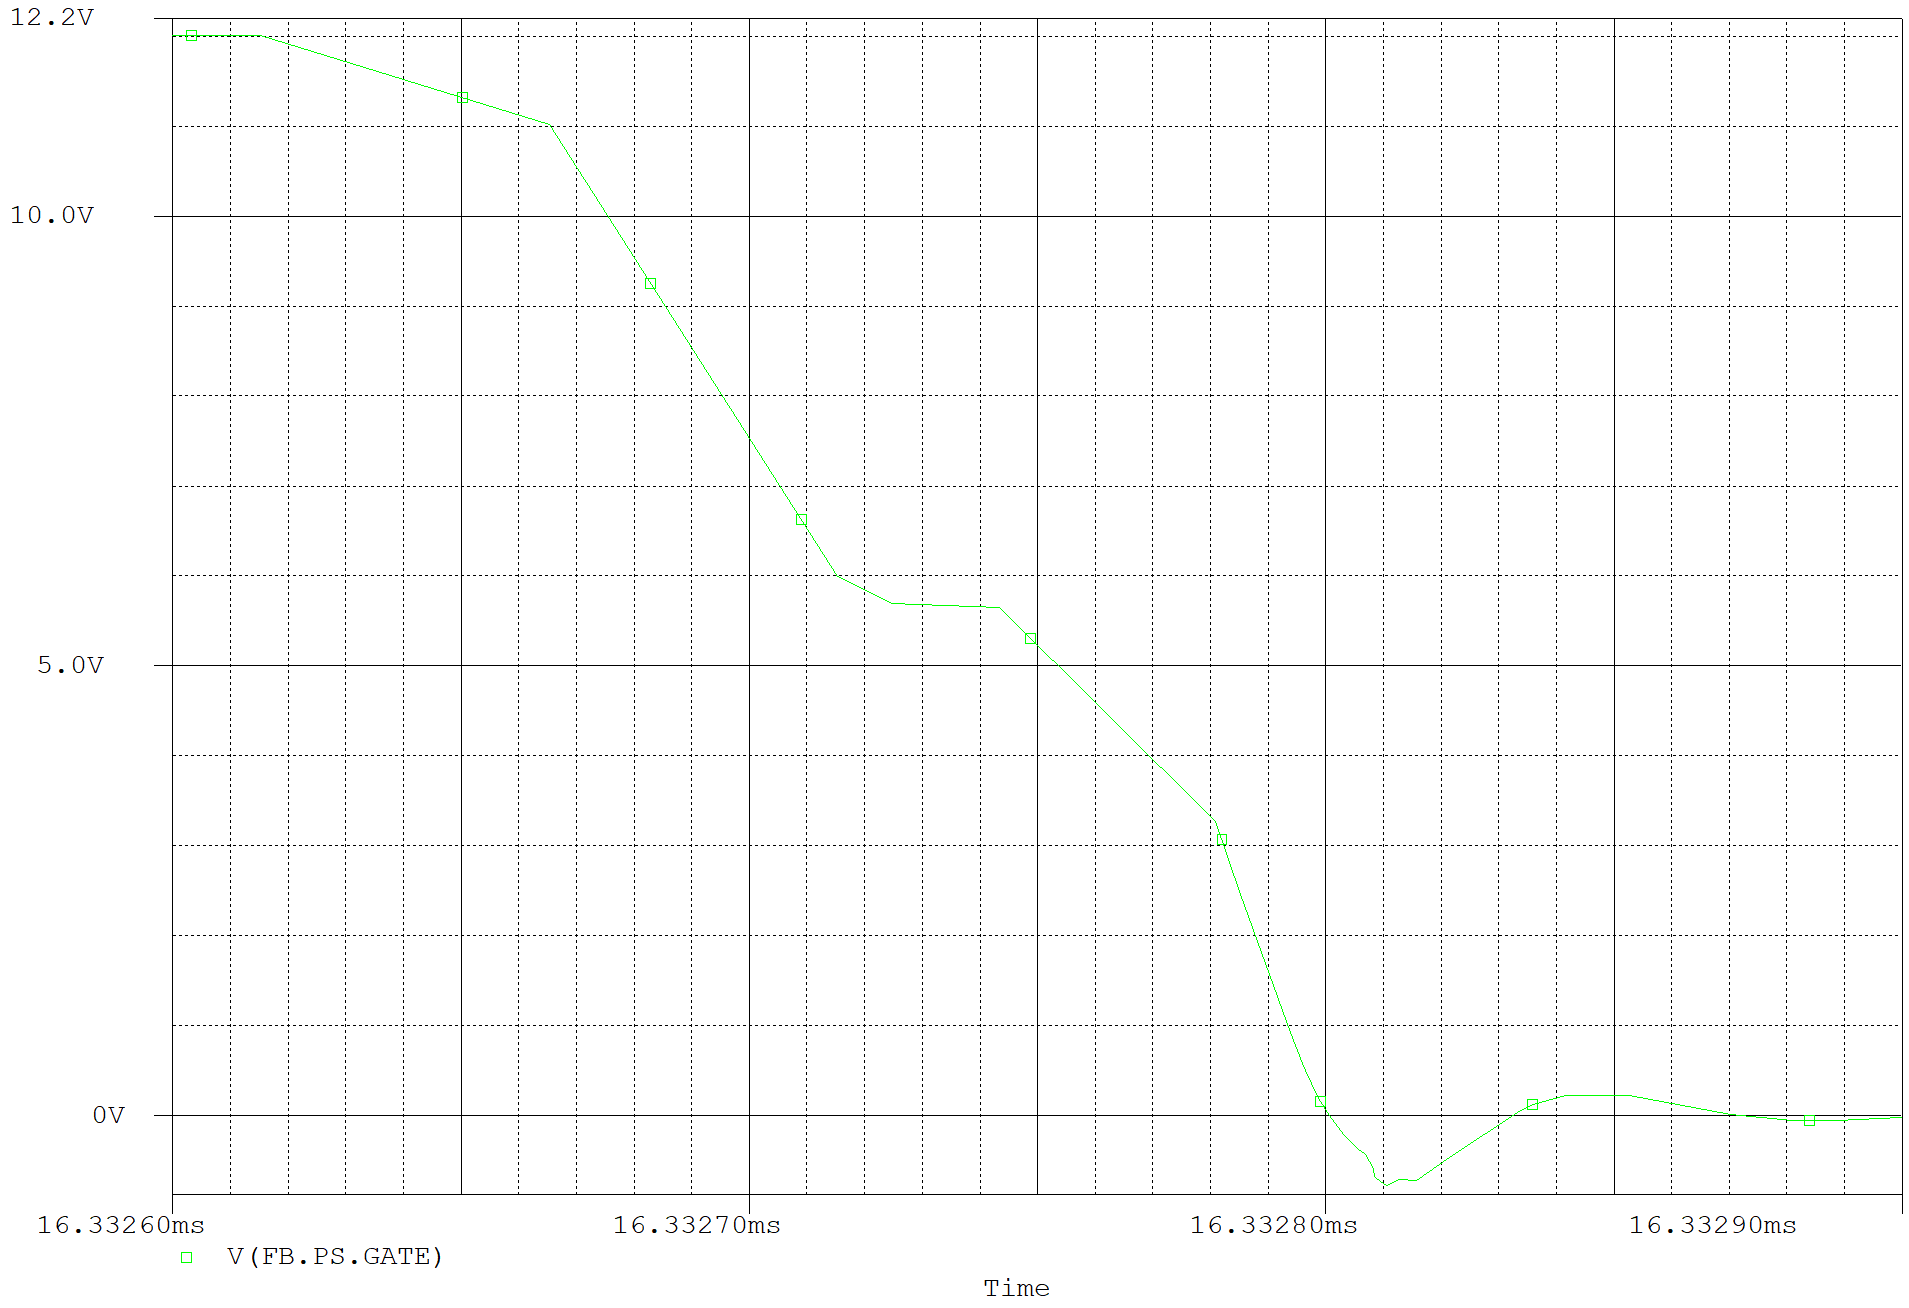
\includegraphics[max width=0.9\linewidth]{/tex/3iteration/billeder/Simulering/Simulering_switch_tid.png}
	\caption{Switch-tid for MOSFET - 3. iteration}
	\label{fig:switch_tid_3}
\end{figure}

\noindent En af konsekvenserne ved en hurtigere switch-tid er, som nævnt i afsnit~\ref{sec:switch_tid}, at peak'en på spændingen over MOSFET'ens drain bliver større. Dette er målt ved figur~\ref{fig:switch_tid_peak}. spændingen aflæses til at have en peak på $110V$. Det er en margin på $27\percent$ til MOSFET'ens breakdown spænding, hvilket godtages. 

\begin{figure}[H]
	\center
	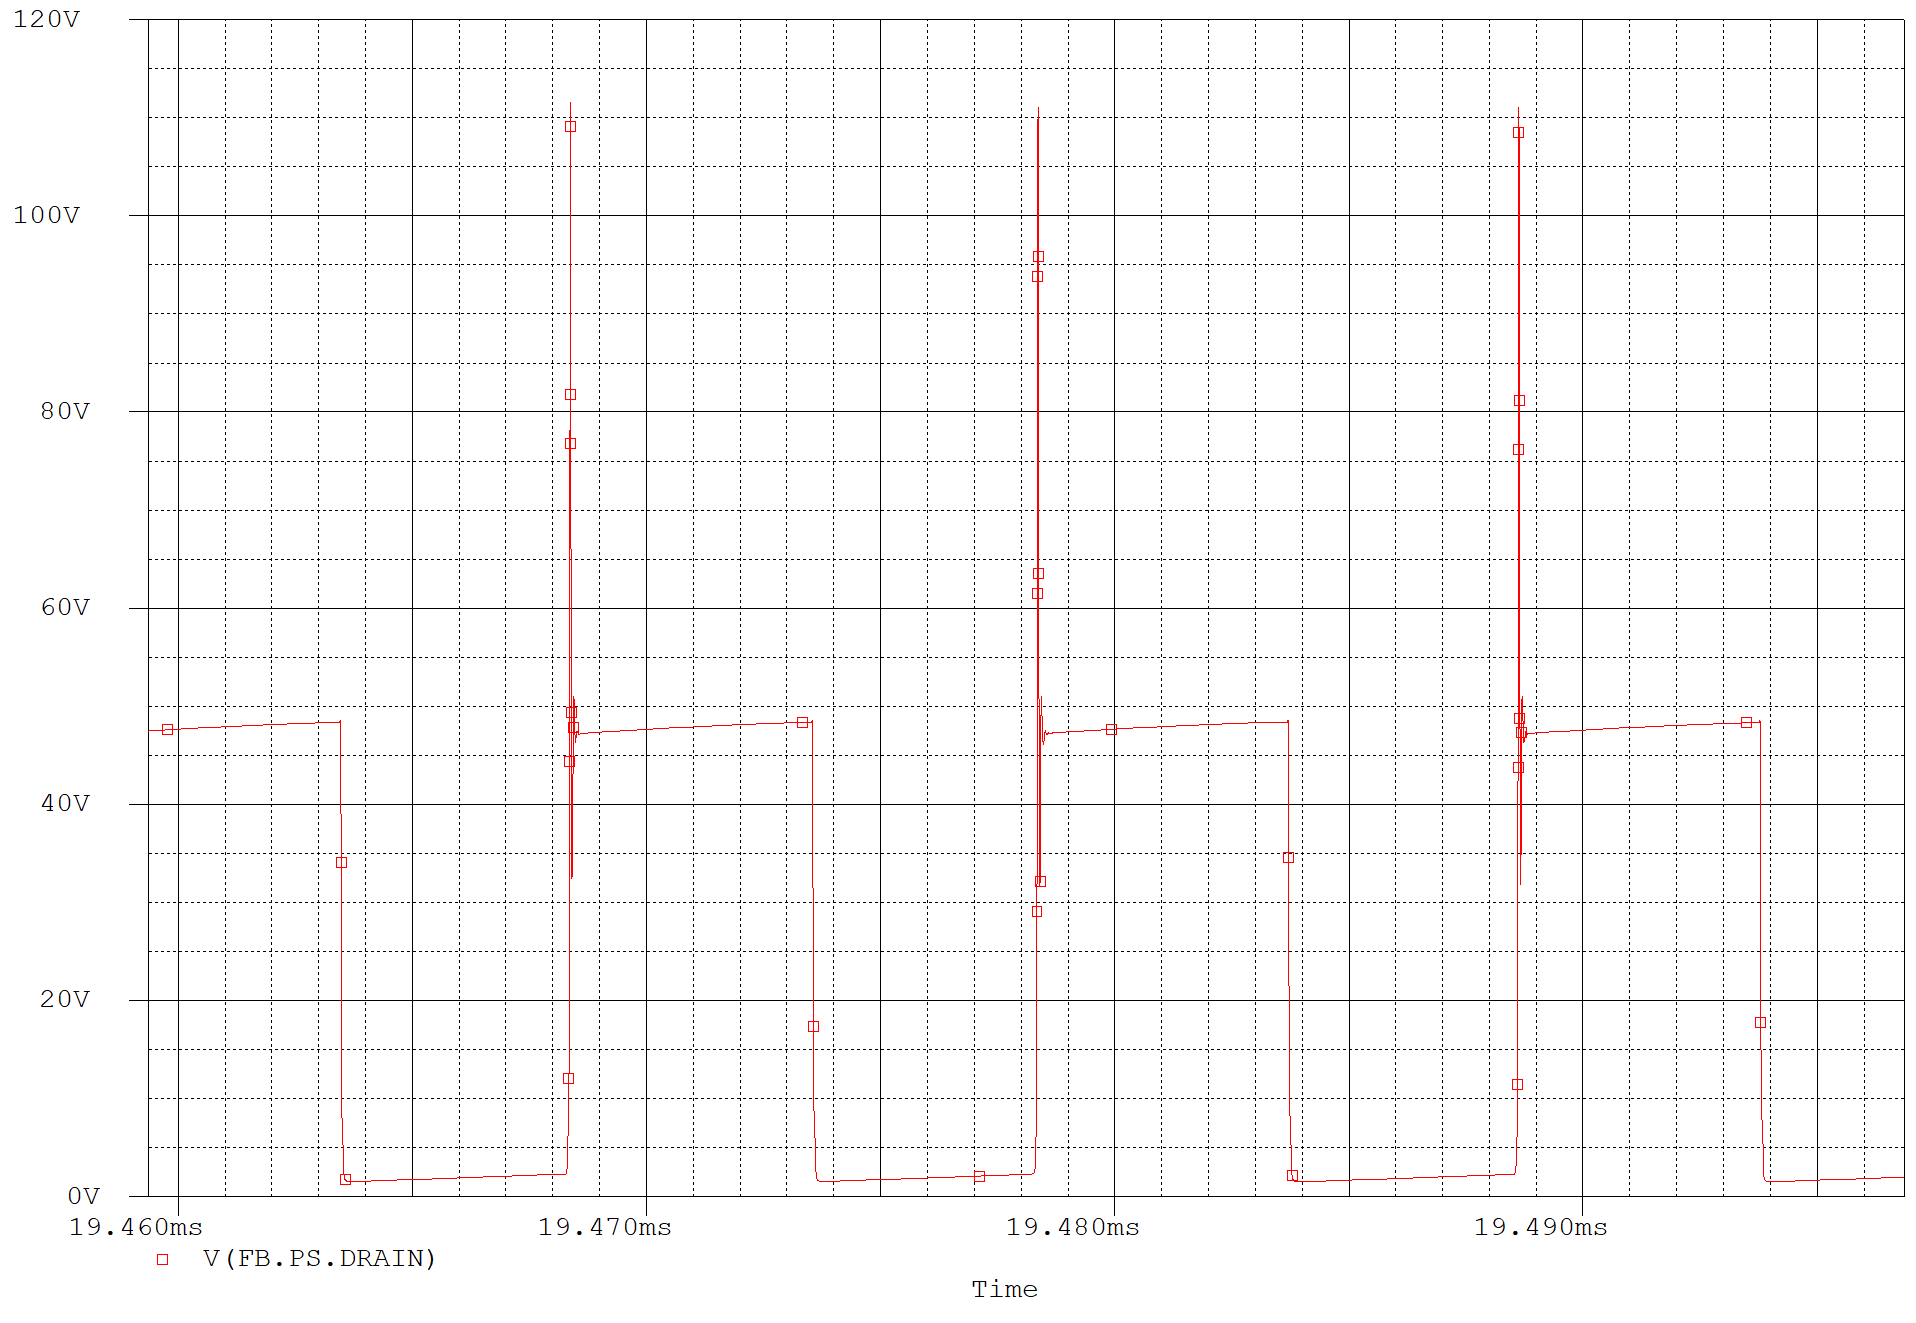
\includegraphics[max width=0.9\linewidth]{/tex/3iteration/billeder/Simulering/Simulering_switch_tid_peak.png}
	\caption{MOSFET drain - 3. iteration}
	\label{fig:switch_tid_peak}
\end{figure}